\subsubsection{Power DCB without backplane}
DCB can be powered by a power breakout board, in the absence of backplane.
The location of the power connector is marked on \autoref{fig:dcb_layout}, with
a label of ``power''.

A un-soldered power breakout board is shown in \autoref{fig:power_breakout}.
Solder 1.5 V, 2.5 V, and sense line onto the board, with appropriate wire
gauges.
Install the power to the marked location and power the DCB with some external
power supply.

\begin{figure}[!ht]
    \centering
    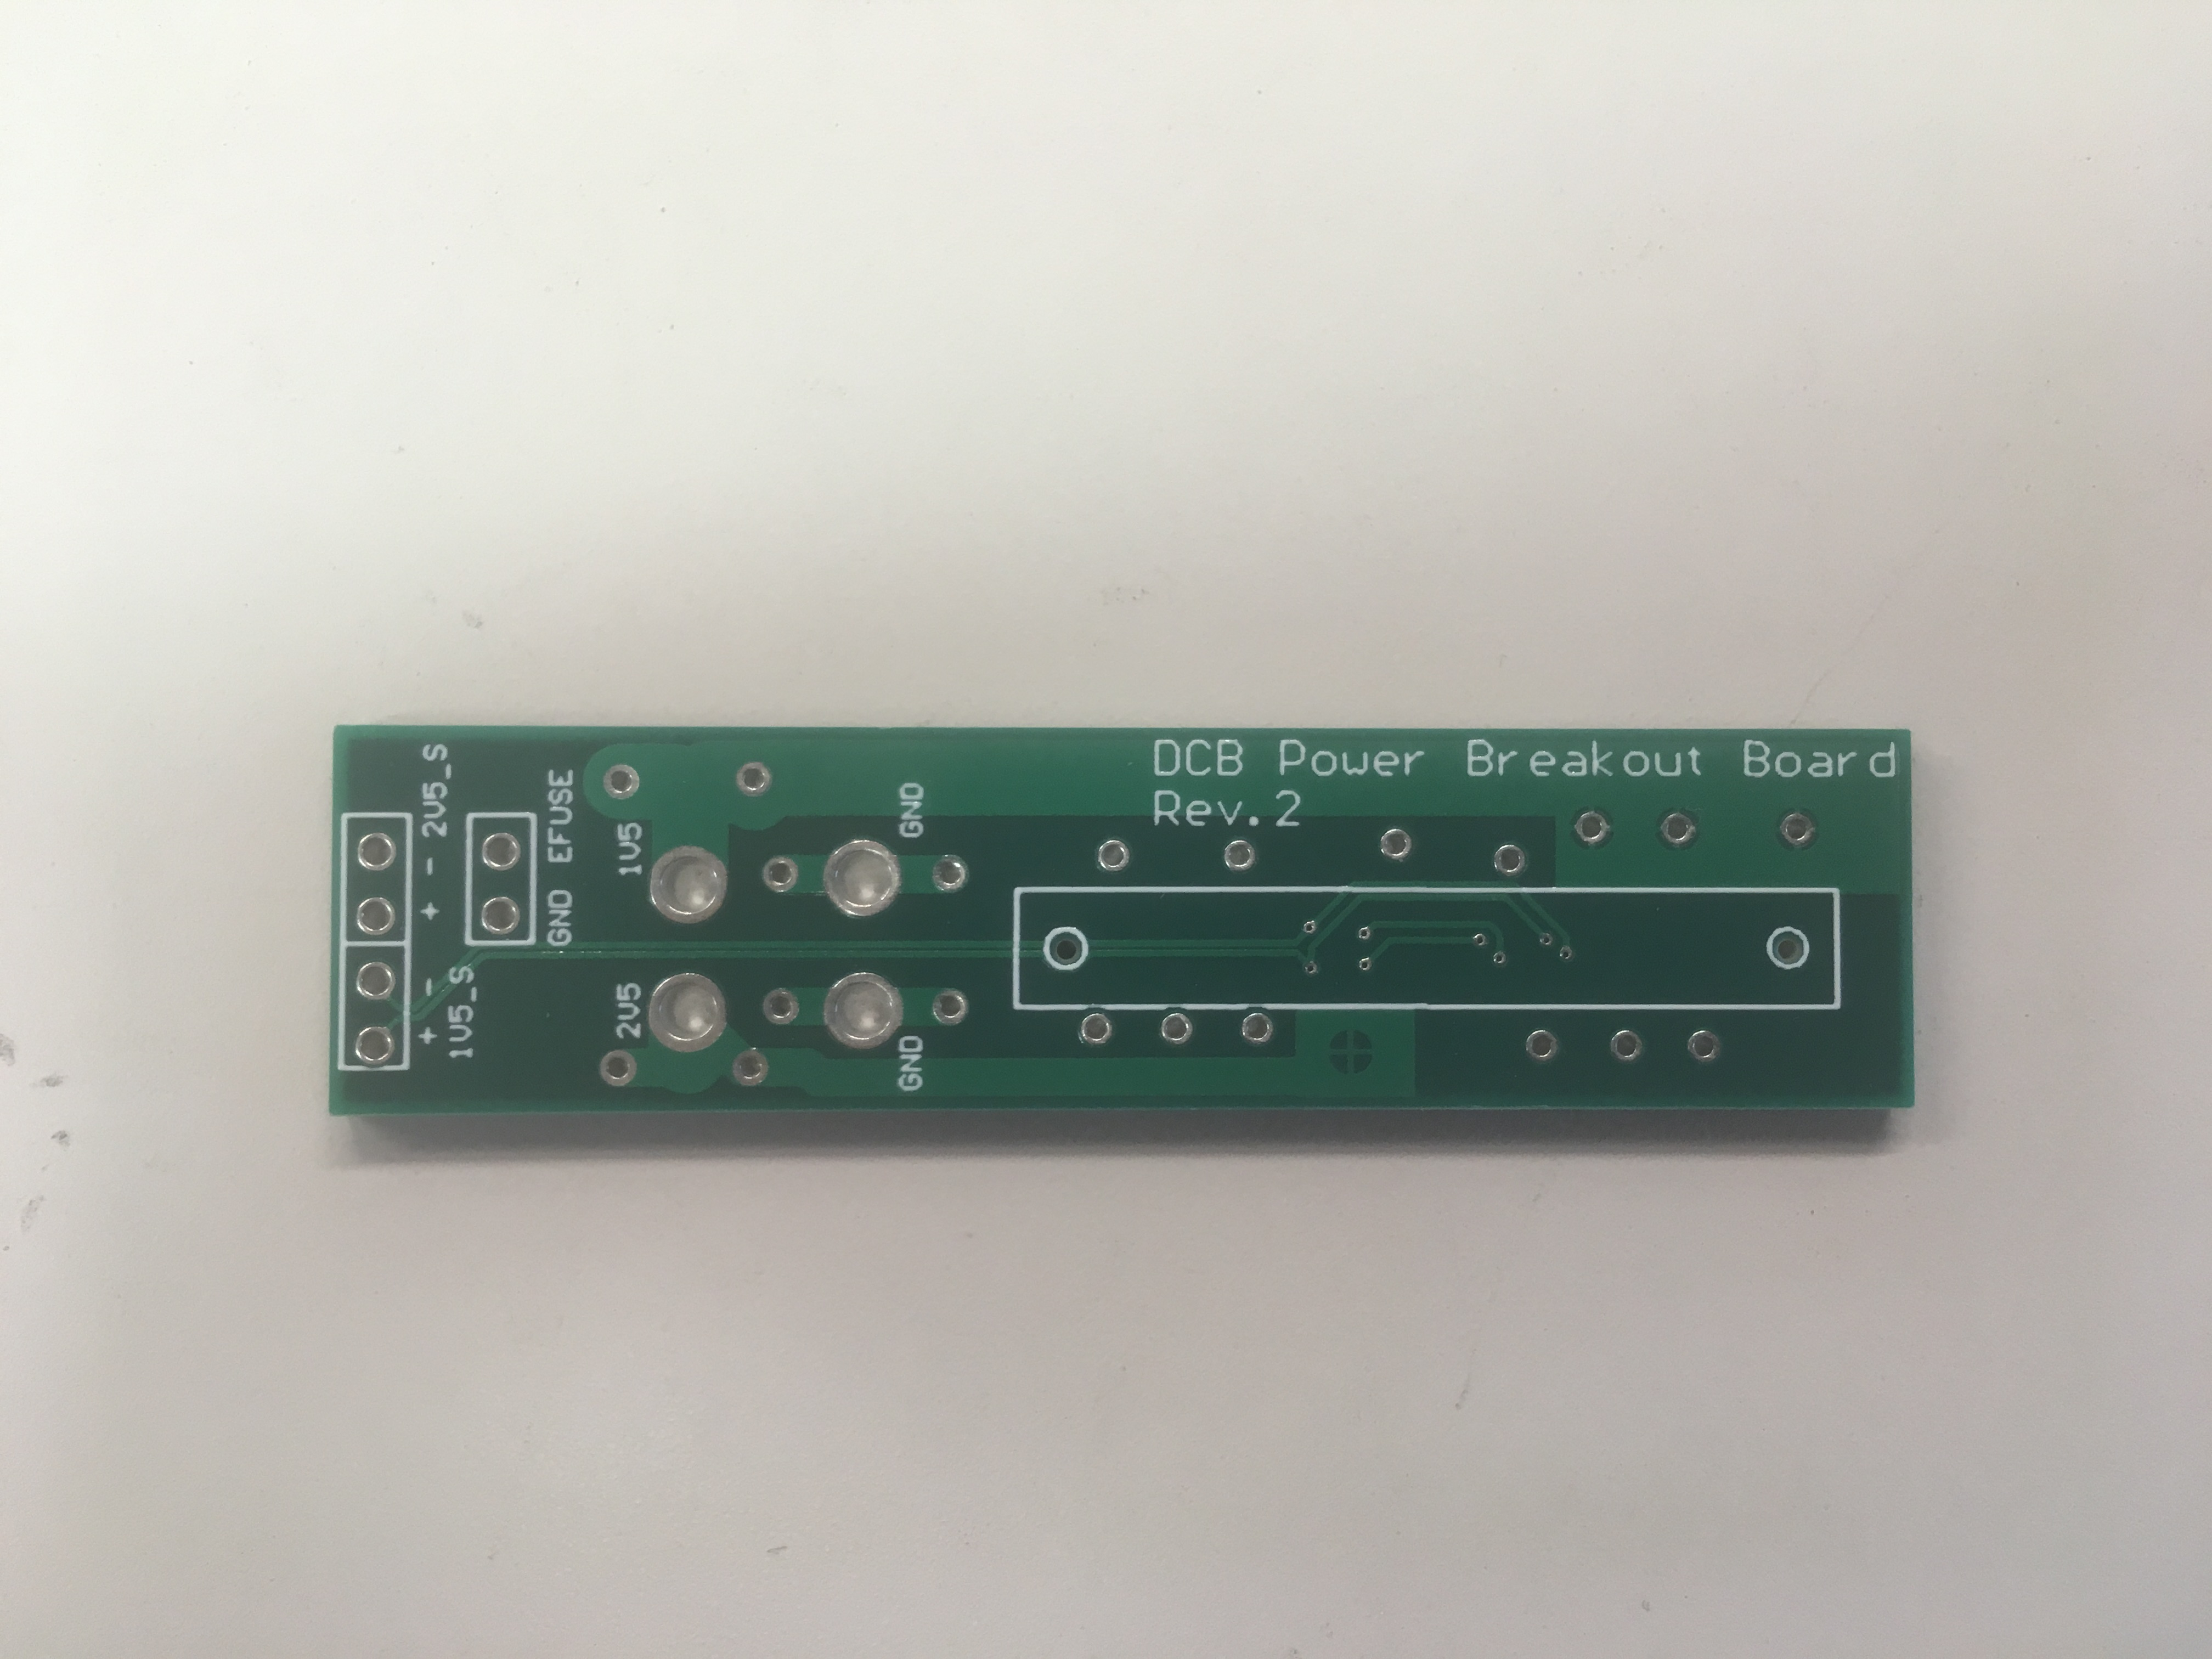
\includegraphics[width=0.9\linewidth]{res/power_breakout_board.jpg}
    \caption{A un-soldered power breakout board.}
    \label{fig:power_breakout}
\end{figure}

\begin{leftbar}
    For 1.5 V rail, it should be able to provide 5 A.
    For 2.5 V, 1 A is sufficient.

    Note that the numbers above are upper bounds, but not the lowest.
    A DCB with master and all 6 data GBTxs configured and idling consumes about
    4.5 A on 1.5 V, and 0.76 A on 2.5 V.
\end{leftbar}
